\chapter{Implementacja}

W niniejszym rozdziale przedstawiono szczegóły techniczne wdrożonego rozwiązania oraz przybliżono aspekty implementacyjne systemu, obejmujące wykorzystanie platformy Microsoft Power Platform -- w szczególności Power Apps -- do budowy interfejsu użytkownika oraz Power Automate do automatyzacji procesów biznesowych.
Ponadto, omówiono integrację z platformą SharePoint oraz implementację skryptów usprawniających pracę z pakietem Microsoft Office.

W ramach analizy technicznej szczegółowo opisano wszystkie komponenty systemu oraz sposób
ich integracji. Szczególną uwagę poświęcono mechanizmom przepływu danych, automatyzacji procesów oraz implementacji logiki biznesowej w środowisku Low-Code.

\section{Utworzenie bazy danych na platformie Sharepoint}

Zgodnie z koncepcją, baza danych utworzona została w środowisku SharePoint.
Pierwszym krokiem było stworzenie strony dedykowanej temu procesowi. Jest to niezwykle proste. W ekranie startowym programu należy wybrać opcję \emph{Utwórz witrynę}. Następnie należy wybrać typ witryny \emph{Witryna zespołu} oraz szablon określający jej wygląd. Na koniec należy określić nazwę tworzonej strony.

Kolejnym krokiem jest utworzenie struktury list oraz plików. Na potrzeby procesu utworzono dwa foldery -- \emph{TempFiles} przechowujący arkusze przed zapisaniem ich danych na listach oraz \emph{ArchivedFiles} przechowujący pliki po zakończeniu procesu.
Ponadto utworzono trzy listy:
\begin{itemize}
    \item \emph{Lista\_Uslug},
    \item \emph{Lista\_Kwot},
    \item \emph{Lista\_Indykacji}.
\end{itemize}
Ich struktura jest taka sama jak opisana w podsekcji \ref{Subsec: StrukturaBazyDanych}. 
W celu dodania tych elementów należy wejść w utworzoną witrynę, następnie wybrać \emph{Zawartość witryny} z bocznego paska nawigacji. Dalej, należy wcisnąć przycisk \emph{Nowy} i wybrać typ elementu -- \emph{Lista} oraz \emph{Biblioteka dokumentów}. Na końcu trzbea podać nazwę oraz opcjonalnie opis elementu.
Po wykonaniu tych kroków, folder jest gotowy do użycia. Jednakże w przypadku list należy jeszcze zdefiniować kolumny. W tym celu należy wejść w utworzoną listę i wybrać przycisk \emph{Dodaje kolumnę} znajdujący się po prawej stronie domyślnie utworzonych kolumn. Dalej pojawi się okno z możliwością wyboru typu kolumny oraz jej nazwy. Po zatwierdzeniu, kolumna zostanie dodana do listy.
Na koniec należy skonfigurować niektóre kolumny. Aby to zrobić należy wybrać ustawienia strony i nacisnąć pozycję \emph{Ustawienia listy}. Tam wybieramy nazwę kolumny, którą chcemy skofigurować.\\
Tabela \ref{tab:SharepointList} przedstawia konfigurację listy:
\begin{table}[t]
    \centering
    \caption{Konfiguracja listy na platformie Sharepoint}
    \label{tab:SharepointList}
\begin{tabular}{|l|l|}
    \hline
    \textbf{Nazwa kolumny} & \textbf{Typ} \\ \hline
    Service\_ID & Liczba \\ \hline
    Service\_Name & Pojedynczy wiersz tekstu \\ \hline
    Service\_Group & Pojedynczy wiersz tekstu \\ \hline
    Service\_Sub\_Group & Pojedynczy wiersz tekstu \\ \hline
    Service\_Main\_Group & Pojedynczy wiersz tekstu \\ \hline
    Instruction\_Link & Pojedynczy wiersz tekstu \\ \hline
    Unit\_Of\_Measurement & Pojedynczy wiersz tekstu \\ \hline
    Settlement\_Type & Pojedynczy wiersz tekstu \\ \hline
    Business\_Service\_Manager & Pojedynczy wiersz tekstu \\ \hline
    Current\_Year\_Plan\_EUR & Liczba \\ \hline
    QTY\_Current\_Year & Liczba \\ \hline
    Next\_Year\_Plan\_EUR & Liczba \\ \hline
    QTY\_Next\_Year & Liczba \\ \hline
    Difference & Obliczeniowa \\ \hline
    MPK & Pojedynczy wiersz tekstu \\ \hline
    Year & Liczba \\ \hline
    IndicationNo & Liczba \\ \hline
    Comment\_Date & Pojedynczy wiersz tekstu \\ \hline
    Comment\_Author & Wiele wierszy tekstu \\ \hline
    Comment\_PZ\_to\_WOB & Wiele wierszy tekstu \\ \hline
    Comment\_BSM & Wiele wierszy tekstu \\ \hline
    Comment\_K-DES & Wiele wierszy tekstu \\ \hline
    Comment\_Intern & Wiele wierszy tekstu \\ \hline
    Decision & Liczba \\ \hline
    Final\_comment & Wiele wierszy tekstu \\ \hline
    \end{tabular}
\end{table}

    \noindent Kolumna \emph{Difference} jest kolumną obliczeniową co oznacza, że jej wartość jest obliczana względem podanej formuły. W tym przypadku oblicza ona różnicę cen między rokiem następnym a bieżącym. \\
    Kolumna \emph{MPK} pomimo wartości liczbowych, jest typu tekstowego gdyż znacznie upraszcza to filtrowanie oraz przepisywanie istniejących numerów do nowych danych. \\
    Kolumna \emph{Decision} jest kolumną liczbową ponieważ status decyzji konwertowany jest na kod liczbowy aby przyspieszyć proces filtrowania:
    \begin{itemize}
        \item \emph{Accepted} $\rightarrow$ 1,
        \item \emph{Not Accepted} $\rightarrow$ -1,
        \item \emph{No Status} $\rightarrow$ 0.
    \end{itemize}
    


\section{Ekran zapisu danych}

Zdecydowano, że pierwszym ekranem aplikacji będzie ekran zapisu danych. Decyzja ta wynika z faktu, że bez prztworzonych danych, utworzenie innych ekranów byłoby zdecydowanie trudniejsze. Ekran ten składa się z elementów, które zostaną omówione poniżej.

\subsection{Zapis pliku w chmurze}
Pierwszym krokiem jest zapis pliku w chmurze w celu udostepnienia go innym systemom. W tym celu wykorzystano kontrolkę\footnote{Kontrolka -- element służący do nawigacji, wyświetlania danych i obsługi aplikacji.} \emph{Attachment Control}. Pozwala ona na zapisanie pliku w pamięci aplikacji. Odbywa się to przez naciśnięcie przycisku \emph{"Dołącz plik"} lub przy użyciu mechaniki \emph{przeciągnij i upuść} (\english{Drag And Drop}). 

Aby przekazać plik oraz jego zawartość należy nacisnąć przycisk opisany jako \emph{Save attachments} znajdujący się pod wcześniej omawianym elementem. Naciścięcie go skutkuje wywołaniem szeregu funkcji opisanych we właściwości \emph{OnSelect}. W pierwszej kolejności sprawdzane jest, czy plik został załadowany. Jeśli tak, to wywoływany jest przepływ \emph{SaveFileAndRunScript}. Wynik przepływu jest zapisywany w zmiennej tablicowej, która w Power Apps określana jest jako \definicja{kolekcja}, o nazwie \emph{FlowOutput}. Po wykonaniu się przepływu, zapisane w kontrolce pliki są usuwane.

\subsubsection{Przepływ SaveFileAndRunScript}
Przepływ \emph{SaveFileAndRunScript} jest odpowiedzialny za zapisanie pliku w chmurze. W momencie wywołania przepływu plik jest przekazany jako parametr wejściowy. Przepływ ten składa się z kilku kroków, które zostaną omówione w kolejności ich wykonywania.

\begin{figure}[H]
    \centering
    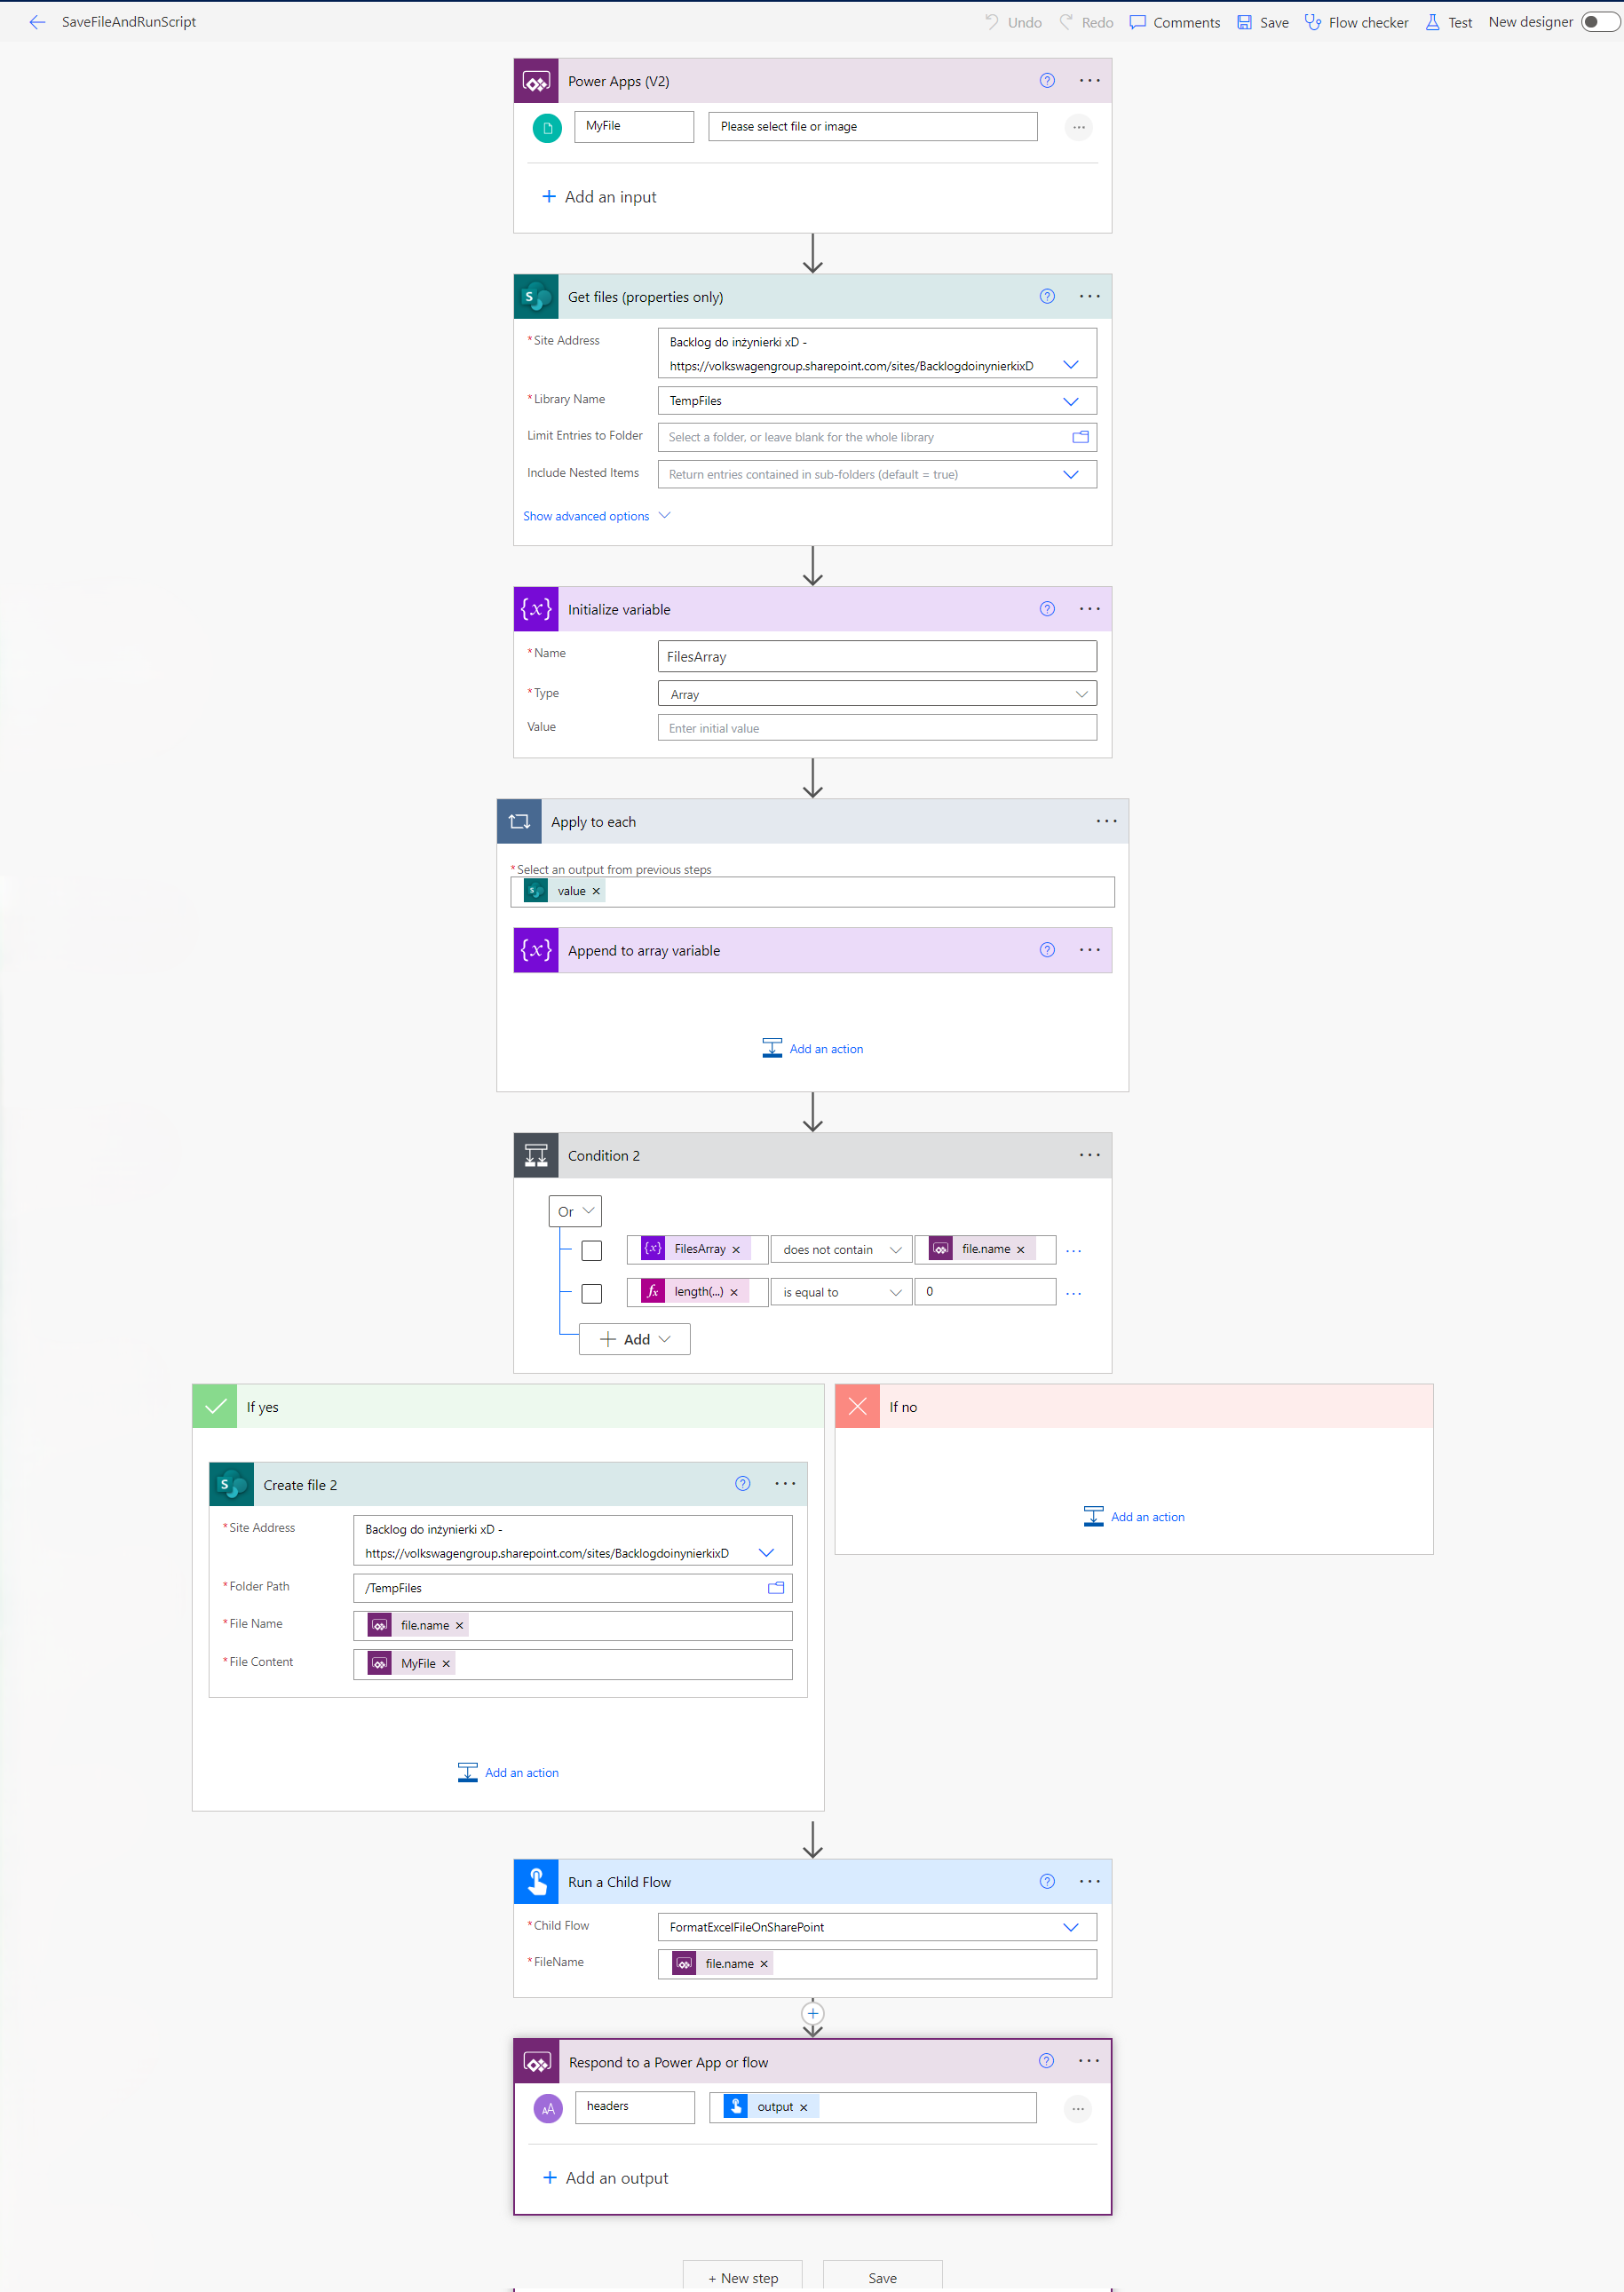
\includegraphics[width=0.85\textwidth]{figures/SaveFileAndRunScript.png}
    \caption{Widok przepływu SaveFileAndRunScript}
    \label{fig:savefileandrunscript}
\end{figure}

Rysunek \ref{fig:savefileandrunscript}, przedstawia widok przepływu \emph{SaveFileAndRunScript}. Przepływ ten składa się z następujących kroków:
\begin{enumerate}
    \item \textbf{Funkcja: Power Apps (V2)} \\
    Jest to element rozpoczynający przepływ, wywoływany bezpośrednio z aplikacji Power Apps. Parametrami wejściowymi są:
    \begin{itemize}
        \item nazwa pliku (\textit{File Name}),
        \item zawartość pliku (\textit{File Content}) w formacie binarnym.
    \end{itemize}

    \item \textbf{Sprawdzenie istniejących plików} \\
    Blok \textit{Get files (properties only)} pobiera listę wszystkich plików z wybranego folderu SharePoint wraz z ich metadanymi, takimi jak nazwa, ścieżka czy data modyfikacji. Pozwala to na sprawdzenie, czy plik o podanej nazwie już istnieje w bibliotece.

    \item \textbf{Warunek} \\
    Element \textit{Condition} sprawdza, czy istnieje plik o nazwie przekazanej w danych wejściowych. W zależności od wyniku:
    \begin{itemize}
        \item jeśli plik istnieje -- przepływ kończy działanie,
        \item jeśli plik nie istnieje -- kontynuuje proces zapisu.
    \end{itemize}

    \item \textbf{Utworzenie pliku} \\
    Blok \textit{Create file} tworzy nowy plik w SharePoint, wykorzystując parametry:
    \begin{itemize}
        \item adres witryny SharePoint,
        \item ścieżkę do folderu docelowego,
        \item nazwę pliku,
        \item zawartość pliku.
    \end{itemize}

    \item \textbf{Uruchomienie podprzepływu} \\
    Element \textit{Run a Child Flow} wywołuje skrypt Office Script, który:
    \begin{itemize}
        \item analizuje zapisany plik,
        \item sprawdza jego zawartość,
        \item formatuje dane według wymagań,
        \item zwraca wynik w formacie JSON.
    \end{itemize}

    \item \textbf{Odpowiedź do aplikacji} \\
    Blok \textit{Respond to Power Apps} kończy przepływ, zwracając do aplikacji dane w formacie JSON przetworzone przez wcześniej wspomniany skrypt Office Script.
\end{enumerate}

\subsection{Skrypt Office Script}
Po utworzeniu pliku w SharePoint, w ramach przepływu następuje jego przetworzenie przez skrypt Office Script. W tym przypadku skrypt ma za zadanie przeanalizować plik i dostosować go do wymagań systemu. Poniżej przedstawiono kroki działania skryptu:

\begin{enumerate}
    \item \textbf{Inicjalizacja i wybór arkusza}
    \begin{itemize}
        \item sprawdzenie wszystkich arkuszy w pliku Excel,
        \item wybór arkusza zawierającego dane,
        \item sprawdzenie i ewentualne usunięcie ochrony hasłem.
    \end{itemize}

    \item \textbf{Analiza danych}
    \begin{itemize}
        \item sprawdzenie czy dane są zorganizowane w tabeli,
        \item w przypadku braku tabeli -- utworzenie nowej,
        \item automatyczne uzupełnienie pustych miejsc w ważnych kolumnach.
    \end{itemize}

    \item \textbf{Dopasowanie nazw kolumn}
    \begin{itemize}
        \item porównanie istniejących nazw kolumn ze standardową listą,
        \item wykorzystanie algorytmu \emph{Jaro-Winkler} do oceny podobieństwa tekstu,
        \item automatyczne rozpoznawanie podobnych nazw (np. "Srv ID" jako "Service ID"),
        \item sugestia ręcznego wyboru przy zbyt małym podobieństwie (poniżej 90\%).
    \end{itemize}

    \item \textbf{Przekazanie wyników}
    \begin{itemize}
        \item zwrócenie oryginalnych nazw kolumn z pliku,
        \item zwrócenie dopasowanych standardowych nazw kolumn,
        \item w razie problemów - przekazanie odpowiednich komunikatów błędów.
    \end{itemize}
\end{enumerate}


\vspace{1cm}
Po zakończeniu działania skryptu Office Script i całego przepływu, przetworzony plik zostaje w pełni zapisany w bibliotece SharePoint. 
Rysunek \ref{fig:saveattachmentsform} przedstawia wspomnianą wcześniej kontrolkę \emph{Attachment Control}, przycisk \emph{Save attachments} oraz listę plików zapisanych w foldrze SharePoint.


\begin{figure}[h]
    \centering
    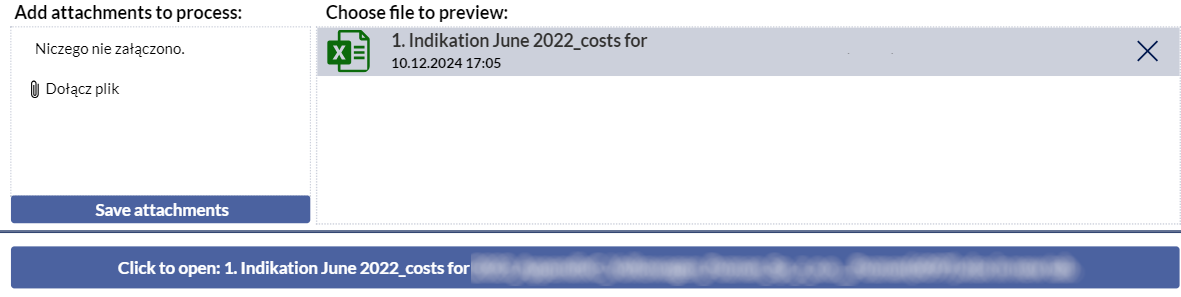
\includegraphics[width=\textwidth]
    {figures/SaveAttachmentsForm.png}
    \caption{Formularz zapisu pliku}    
    \label{fig:saveattachmentsform}
\end{figure}

Wybór elementu z listy \emph{Choose file to preview} umożliwia wskazanie pliku do dalszego przetwarzania. Selekcja pozycji z listy automatycznie inicjuje wykonanie opisanego wcześniej skryptu, którego celem jest pozyskanie aktualnego zestawu nagłówków. Należy podkreślić, że ten sam proces zachodzi również podczas inicjalizacji aplikacji. 
Funkcjonalność podglądu, zaimplementowana w postaci przycisku umiejscowionego poniżej głównych elementów sterujących, umożliwia otwarcie wybranego pliku w nowej karcie przeglądarki. Jest to szczególnie istotne w kontekście weryfikacji poprawności danych oraz walidacji struktury kolumn.
\section{Edycja danych}

Po wstępnym podegraniu pliku źródłowego, następnym krokiem jest umożliwienie użytkownikom modyfikacji danych w celu wprowadzenia niezbędnych aktualizacji dotyczących usług. W związku z tym utworzono dwa ekrany -- pierwszy służy do wyboru usługi z listy, a drugi umożliwia jej edycję oraz przedstawia niezbędne szczegóły.

\subsection{Ekran wyboru usługi do edycji}

\begin{comment}

Ekran wyboru elementu do obróbki składa się z: \begin{enumerate}
   \item listy, przedstawiającej dane z tymczasowej kolekcji \textit{MergedData}, utworzonej specjalnie na potrzeby obsługi wyboru danych do edycji,
   \item pól wyszukiwania i filtrów, umożliwiających zawężenie listy na podstawie nazwy usługi, identyfikatora (\textit{Service ID}), miejsca powstawania kosztów (\textit{MPK}) oraz statusu decyzji (\textit{Accepted}, \textit{Not Accepted}, \textit{No Status}),
   \item wykresu kołowego, prezentującego wizualne podsumowanie liczby elementów w każdej kategorii statusu decyzji,
   \item interfejsu umożliwiającego dynamiczne dopasowanie wyników listy w czasie rzeczywistym, na podstawie wprowadzonych kryteriów wyszukiwania,
   \item nagłówka, który przedstawia kontekst użytkownika, w tym nazwę i dane aktualnie zalogowanego użytkownika. \end{enumerate}
\end{comment}

\subsubsection*{Lista danych}
Lista prezentuje dane pochodzące z dynamicznej kolekcji \textit{MergedData}, która została utworzona w celu zintegrowania informacji z trzech różnych list SharePoint (\textit{Lista\_Uslug}, \textit{Lista\_Kwot}, \textit{Lista\_Indykacji}). Dzięki zastosowaniu wbudowanych funkcji \textit{LookUp} (wyszukiwanie pojedynczego elementu w źródle danych na podstawie warunku) oraz \textit{AddColumns} (dodawanie nowych kolumn do istniejącego źródła danych), dane są filtrowane tak, aby wyświetlać jedynie najnowsze rekordy, np. dla najświeższych decyzji i kwot. Taka struktura zapewnia użytkownikom dostęp do aktualnych informacji bez konieczności ręcznego przeszukiwania źródłowych list. Lista jest dynamiczna, co oznacza, że zmiany w danych źródłowych są automatycznie uwzględniane.

Każdy element na liście posiada dodatkową funkcję interakcji. Po najechaniu kursorem na wybraną usługę (funkcja \textit{hover}), element wizualnie zmienia swój wygląd -- zwęża się, zmienia kolor oraz staje się możliwy do kliknięcia. Kliknięcie przenosi użytkownika do dedykowanego ekranu edycji, który umożliwia szczegółowe zarządzanie wybraną usługą.

\subsubsection*{Pola wyszukiwania i filtry}
Użytkownik ma możliwość zawężenia widocznych danych poprzez zastosowanie różnych kryteriów wyszukiwania. Pola obejmują:
\begin{itemize}
   \item {Wyszukiwanie po nazwie usługi (\textit{Service Name})} -- Obsługuje częściowe dopasowania dzięki wbudowanej funkcji \textit{StartsWith} (sprawdza, czy ciąg tekstowy zaczyna się od określonej frazy).
   \item {Filtrowanie po identyfikatorze usługi (\textit{Service ID})} -- Umożliwia precyzyjne wyszukiwanie konkretnego elementu.
   \item {Filtrowanie według miejsca powstawania kosztów (\textit{MPK})} -- Pozwala na szybkie odnalezienie danych przypisanych do konkretnego obszaru finansowego.
   \item {Filtrowanie według statusu decyzji (\textit{Accepted}, \textit{Not Accepted}, \textit{No Status})} -- Dzięki zastosowaniu funkcji \textit{Switch} (zwraca wartość w zależności od spełnionego warunku), wartości statusów są mapowane na odpowiednie kody liczbowe.
\end{itemize}
Filtry te mogą być stosowane jednocześnie, co umożliwia precyzyjne dopasowanie wyświetlanych danych.

\subsubsection*{Wykres kołowy}
Wykres kołowy ilustruje podział danych według statusów decyzji. Każdy segment odpowiada liczbie elementów z przypisanym statusem, co pozwala użytkownikowi szybko ocenić proporcje między kategoriami (\textit{Accepted}, \textit{Not Accepted}, \textit{No Status}). Wykres jest dynamiczny -- aktualizuje się w czasie rzeczywistym w oparciu o zastosowane filtry.



\subsection{Ekran edycji elementu}
Ekran edycji elementu prezentuje szczegółowe informacje dotyczące wybranej usługi, umożliwiając analizę danych historycznych oraz wprowadzanie nowych decyzji. Ekran składa się z kilku logicznie ułożonych sekcji, które są opisane poniżej.

\subsubsection{Porównanie finalnych decyzji z poprzednich lat}
W górnej części ekranu znajduje się tabela przedstawiająca porównanie danych finansowych oraz decyzji z trzech ostatnich lat. Dane te są automatycznie pobierane i zawierają:
\begin{itemize}
   \item {Rok (Year)} -- okres, którego dotyczy dana decyzja,
   \item {Jednostka miary (Unit Of Measurement)} -- np. liczba użytkowników lub inne wskaźniki operacyjne,
   \item {Planowane i rzeczywiste wartości finansowe} -- np. \textit{Current Year Plan} oraz \textit{Next Year Plan},
   \item {Różnice w finansach (Difference)} -- różnica między planowanymi i rzeczywistymi kosztami,
   \item {Status końcowej decyzji (Final Decision)} -- decyzje dotyczące planów z danego roku (\textit{Accepted, Not Accepted, No Status}).
\end{itemize}

Sekcja ta pozwala użytkownikowi przeanalizować ostatnie decyzje oraz ocenić trendy finansowe dla danej usługi w kolejnych latach.

\subsubsection{Link do instrukcji obsługi}
Poniżej tabeli z porównaniem decyzji znajduje się link do dedykowanej instrukcji obsługi usługi. Link zapewnia użytkownikowi dostęp do szczegółowych informacji na temat zasad korzystania z danej usługi, co może być przydatne podczas edycji danych lub wprowadzania nowych decyzji.

\subsubsection{Porównanie tegorocznych indykacji}
Sekcja ta prezentuje szczegóły kolejnych indykacji w ramach bieżącego roku. Użytkownik może zobaczyć i analizować szczegóły poszczególnych indykacji, takich jak:
\begin{itemize}
   \item {Numer indykacji (Indication Number)} -- numer kolejny przypisany do konkretnej decyzji,
   \item {Komentarze} -- w tym \textit{Internal Comment, Comment PZ to WOB, Comment K-DES}, które umożliwiają przekazanie informacji pomiędzy działami,
   \item {Data i autor komentarza} -- dane dotyczące daty wprowadzenia decyzji oraz osoby odpowiedzialnej,
   \item {Status decyzji (Decision)} -- użytkownik może zobaczyć, czy decyzja została zaakceptowana (\textit{Accepted}), odrzucona (\textit{Not Accepted}) lub jeszcze nie podjęta (\textit{No Status}).
\end{itemize}

\subsubsection{Formularz do uzupełnienia danych}
Na samym dole strony znajduje się formularz umożliwiający wprowadzenie nowych danych lub aktualizację istniejących rekordów. Formularz zawiera pola takie jak:
\begin{itemize}
   \item {Rok (Year)} -- użytkownik może wybrać rok, którego dotyczy wpis,
   \item {Numer indykacji (Indication Number)} -- kolejny numer przypisany do decyzji,
   \item {Komentarze} -- pola do wprowadzenia uwag wewnętrznych, komentarzy między działami oraz końcowych komentarzy,
   \item {Status decyzji (Decision)} -- lista rozwijana umożliwiająca wybór odpowiedniego statusu (\textit{Accepted, Not Accepted, No Status}),
   \item {Data i autor} -- data oraz osoba odpowiedzialna za wprowadzenie wpisu.
\end{itemize}

Przycisk \textit{Save} umożliwia zapisanie wprowadzonych zmian. Mechanizm ten:
\begin{itemize}
   \item Sprawdza istnienie wcześniejszych indykacji, aby upewnić się, że zachowana jest poprawna kolejność numeracji,
   \item W przypadku istniejącego wpisu -- aktualizuje dane (\textit{Patch}),
   \item W przypadku nowego wpisu -- tworzy nowy rekord (\textit{Defaults}),
   \item Resetuje pola formularza oraz odświeża dane na ekranie, aby uwzględnić ostatnie zmiany,
   \item Informuje użytkownika o powodzeniu lub błędach operacji za pomocą komunikatów (\textit{Notify}).
\end{itemize}

\subsubsection{Podsumowanie}
Ekran edycji elementu został zaprojektowany tak, aby umożliwić użytkownikom zarówno przeglądanie historycznych danych finansowych, jak i łatwe wprowadzanie nowych decyzji lub modyfikację istniejących. Dzięki logicznemu układowi sekcji oraz dynamicznej aktualizacji danych, interfejs wspiera efektywne zarządzanie informacjami dla każdej usługi.

\section{Generowanie raportu}

W następstwie uzupełnienia wymaganych danych możliwe jest...

\begin{comment}
W niniejszym rozdziale przedstawiono szczegóły techniczne zaimplementowanego rozwiązania. Omówione zostaną kluczowe aspekty
implementacyjne systemu, obejmujące wykorzystanie platformy Microsoft Power Platform - w szczególności
Power Apps do budowy interfejsu użytkownika oraz Power Automate do automatyzacji procesów biznesowych.
Ponadto, przedstawiona zostanie integracja z platformą SharePoint oraz implementacja skryptów
usprawniających pracę z pakietem Microsoft Office. Rozdział stanowi techniczne rozwinięcie przyjętych
założeń projektowych, prezentując metodykę realizacji poszczególnych komponentów systemu.

W ramach analizy technicznej zostaną szczegółowo omówione poszczególne komponenty systemu oraz sposób
ich integracji. Szczególna uwaga zostanie poświęcona mechanizmom przepływu danych, automatyzacji
procesów oraz implementacji logiki biznesowej w środowisku low-code. Ponadto poruszono napotkane problemy oraz ich rozwiązania.

\section{Ekran zapisu danych}

Zdecydowano, że pierwszym ekranem aplikacji będzie ekran zapisu danych. Decyzja ta wynika z faktu, że bez prztworzonych danych, utworzenie innych ekranów byłoby zdecydowanie trudniejsze. Ekran ten składa się z elementów, które zostaną omówione poniżej.

\subsection{Zapis pliku w chmurze}
Pierwszym krokiem jest zapis pliku w chmurze w celu udostepnienia go innym systemom. W tym celu wykorzystano kontrolkę\footnote{Kontrolka -- element służący do nawigacji, wyświetlania danych i obsługi aplikacji.} \emph{Attachment Control}. Pozwala ona na zapisanie pliku w pamięci aplikacji. Odbywa się to przez naciśnięcie przycisku \emph{"Dołącz plik"} lub przy użyciu mechaniki \emph{przeciągnij i upuść} (\english{Drag And Drop}). 

Aby przekazać plik oraz jego zawartość należy nacisnąć przycisk opisany jako \emph{Save attachments} znajdujący się pod wcześniej omawianym elementem. Naciścięcie go skutkuje wywołaniem szeregu funkcji opisanych we właściwości \emph{OnSelect}. W pierwszej kolejności sprawdzane jest, czy plik został załadowany. Jeśli tak, to wywoływany jest przepływ \emph{SaveFileAndRunScript}. Wynik przepływu jest zapisywany w zmiennej tablicowej, która w Power Apps określana jest jako \definicja{kolekcja}, o nazwie \emph{FlowOutput}. Po wykonaniu się przepływu, zapisane w kontrolce pliki są usuwane.

\subsubsection{Przepływ SaveFileAndRunScript}
Przepływ \emph{SaveFileAndRunScript} jest odpowiedzialny za zapisanie pliku w chmurze. W momencie wywołania przepływu plik jest przekazany jako parametr wejściowy. Przepływ ten składa się z kilku kroków, które zostaną omówione w kolejności ich wykonywania.

\begin{figure}[H]
    \centering
    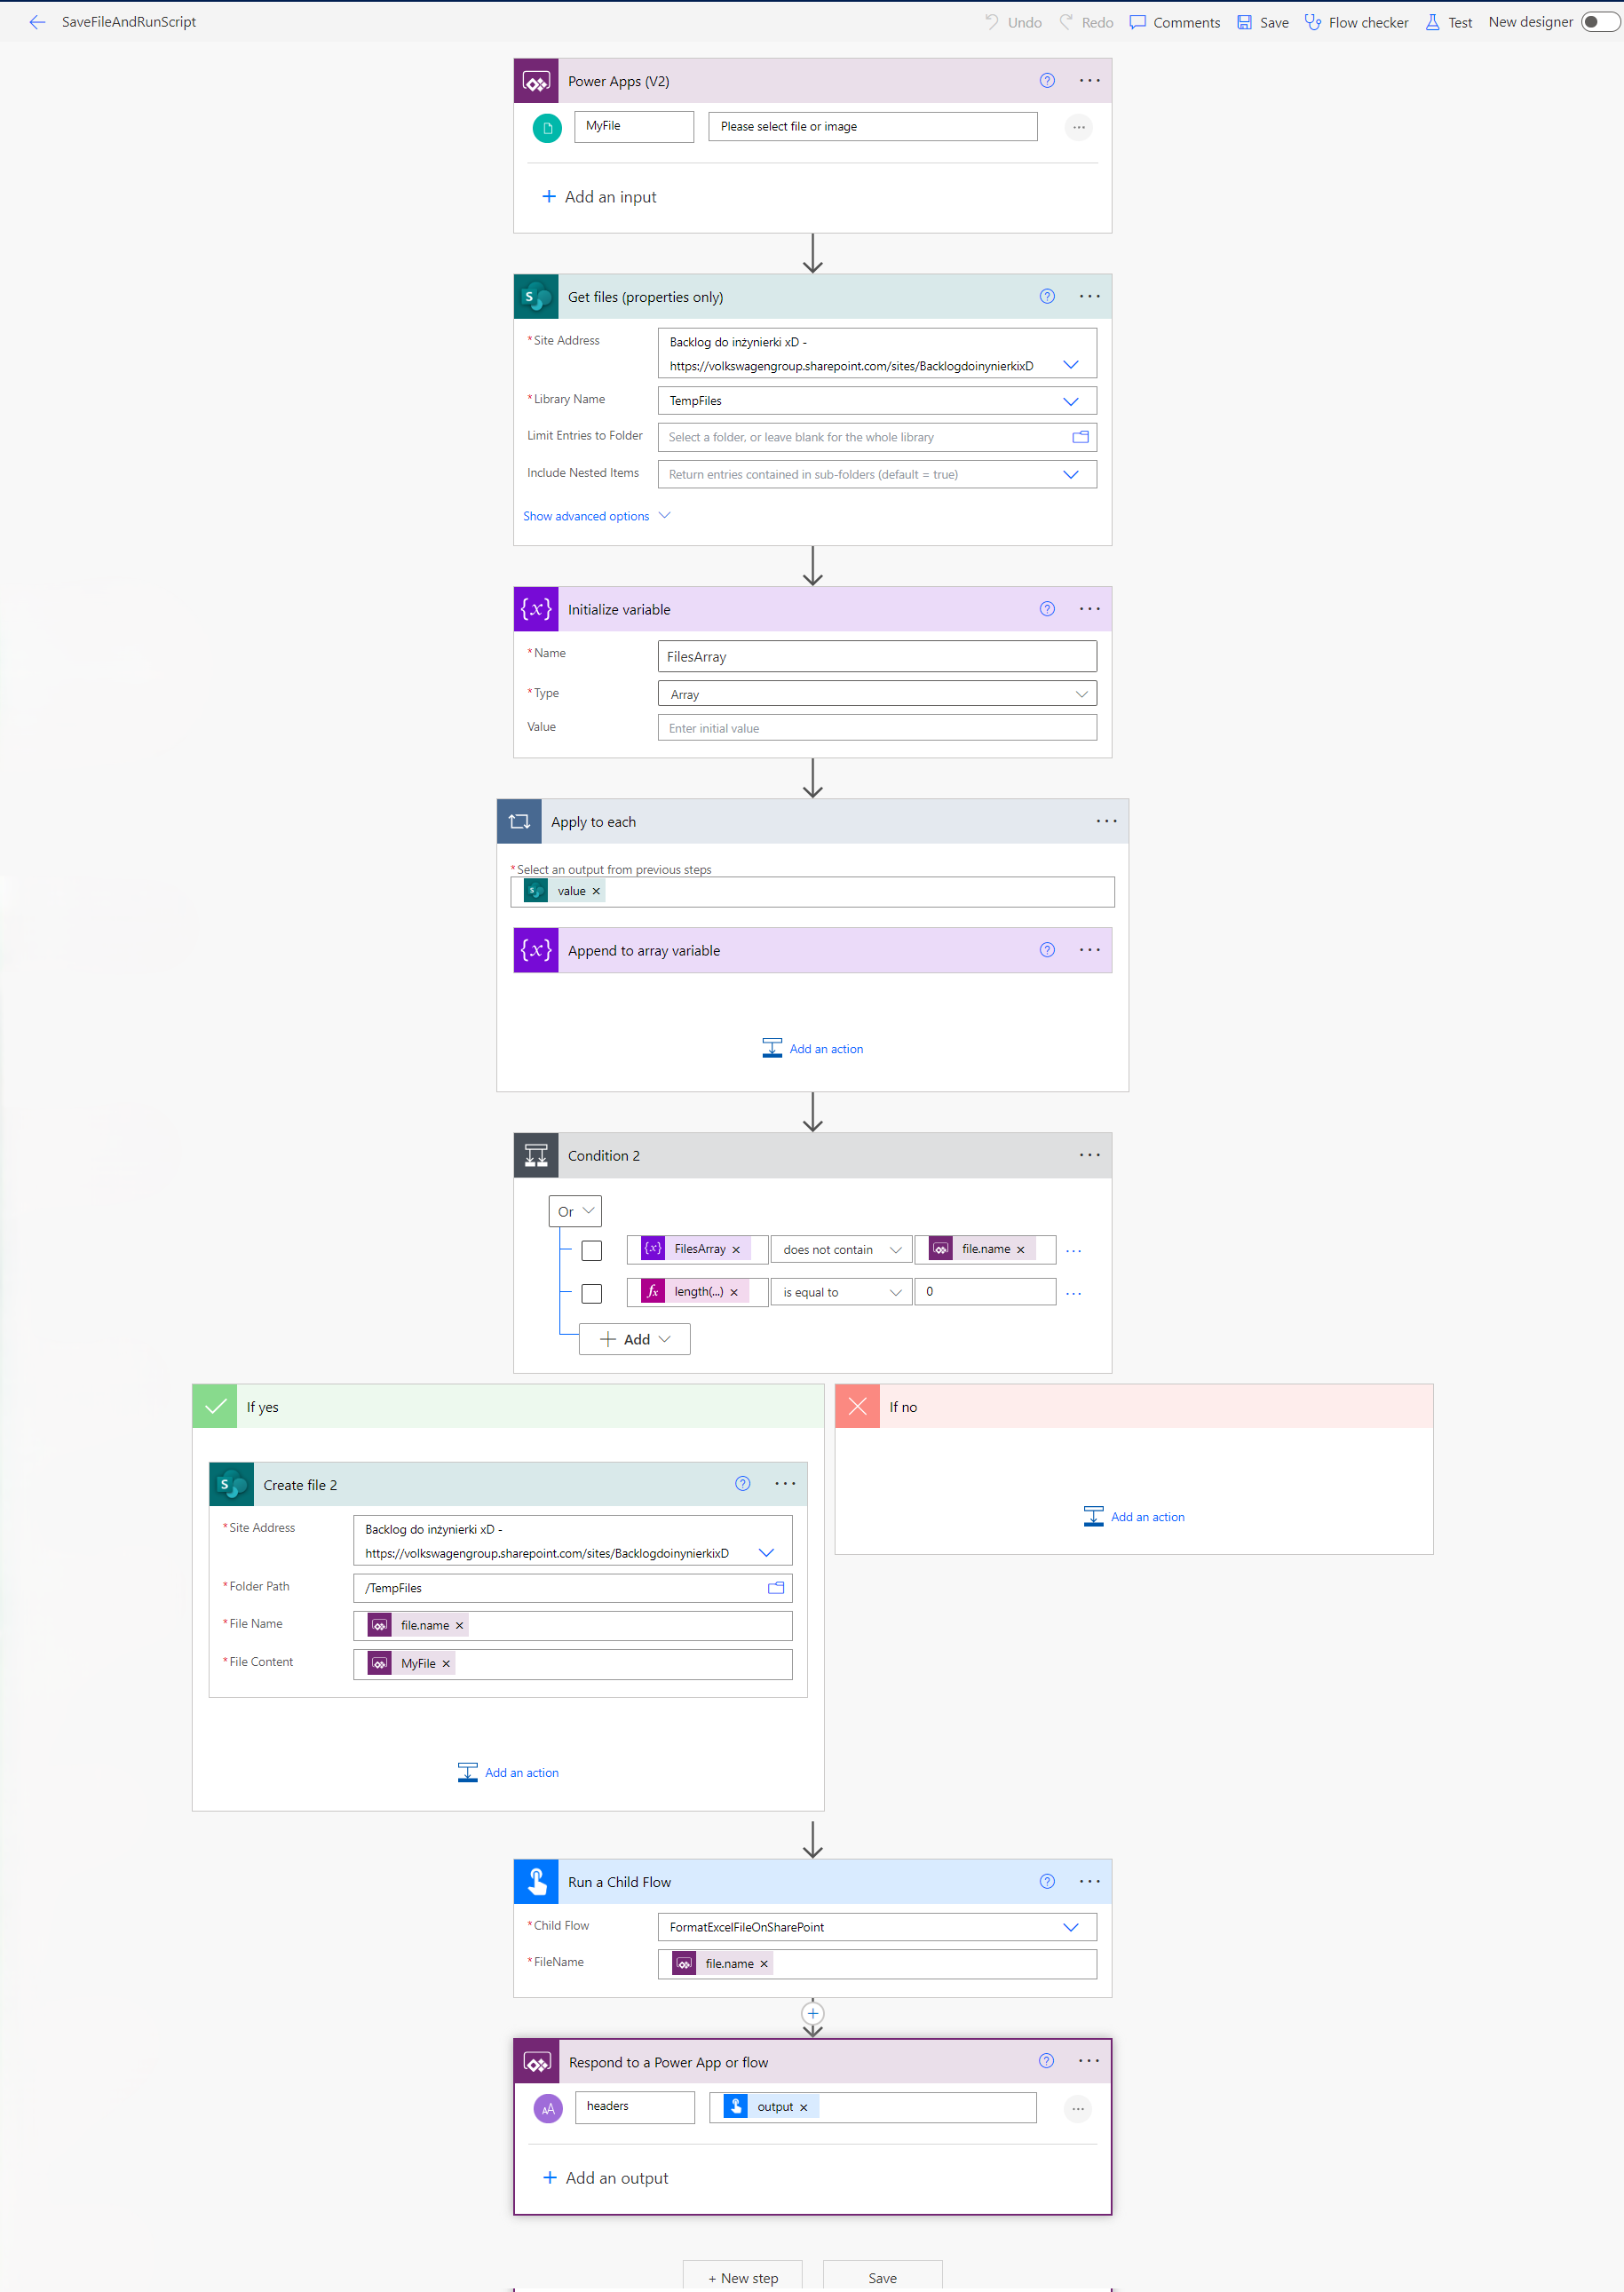
\includegraphics[width=0.85\textwidth]{figures/SaveFileAndRunScript.png}
    \caption{Widok przepływu SaveFileAndRunScript}
    \label{fig:savefileandrunscript}
\end{figure}

Rysunek \ref{fig:savefileandrunscript}, przedstawia widok przepływu \emph{SaveFileAndRunScript}. Przepływ ten składa się z następujących kroków:
\begin{enumerate}
    \item \textbf{Funkcja: Power Apps (V2)} \\
    Jest to element rozpoczynający przepływ, wywoływany bezpośrednio z aplikacji Power Apps. Parametrami wejściowymi są:
    \begin{itemize}
        \item nazwa pliku (\textit{File Name}),
        \item zawartość pliku (\textit{File Content}) w formacie binarnym.
    \end{itemize}

    \item \textbf{Sprawdzenie istniejących plików} \\
    Blok \textit{Get files (properties only)} pobiera listę wszystkich plików z wybranego folderu SharePoint wraz z ich metadanymi, takimi jak nazwa, ścieżka czy data modyfikacji. Pozwala to na sprawdzenie, czy plik o podanej nazwie już istnieje w bibliotece.

    \item \textbf{Warunek} \\
    Element \textit{Condition} sprawdza, czy istnieje plik o nazwie przekazanej w danych wejściowych. W zależności od wyniku:
    \begin{itemize}
        \item jeśli plik istnieje -- przepływ kończy działanie,
        \item jeśli plik nie istnieje -- kontynuuje proces zapisu.
    \end{itemize}

    \item \textbf{Utworzenie pliku} \\
    Blok \textit{Create file} tworzy nowy plik w SharePoint, wykorzystując parametry:
    \begin{itemize}
        \item adres witryny SharePoint,
        \item ścieżkę do folderu docelowego,
        \item nazwę pliku,
        \item zawartość pliku.
    \end{itemize}

    \item \textbf{Uruchomienie podprzepływu} \\
    Element \textit{Run a Child Flow} wywołuje skrypt Office Script, który:
    \begin{itemize}
        \item analizuje zapisany plik,
        \item sprawdza jego zawartość,
        \item formatuje dane według wymagań,
        \item zwraca wynik w formacie JSON.
    \end{itemize}

    \item \textbf{Odpowiedź do aplikacji} \\
    Blok \textit{Respond to Power Apps} kończy przepływ, zwracając do aplikacji dane w formacie JSON przetworzone przez wcześniej wspomniany skrypt Office Script.
\end{enumerate}

\subsection{Skrypt Office Script}
Po utworzeniu pliku w SharePoint, w ramach przepływu następuje jego przetworzenie przez skrypt Office Script. W tym przypadku skrypt ma za zadanie przeanalizować plik i dostosować go do wymagań systemu. Poniżej przedstawiono kroki działania skryptu:

\begin{enumerate}
    \item \textbf{Inicjalizacja i wybór arkusza}
    \begin{itemize}
        \item sprawdzenie wszystkich arkuszy w pliku Excel,
        \item wybór arkusza zawierającego dane,
        \item sprawdzenie i ewentualne usunięcie ochrony hasłem.
    \end{itemize}

    \item \textbf{Analiza danych}
    \begin{itemize}
        \item sprawdzenie czy dane są zorganizowane w tabeli,
        \item w przypadku braku tabeli -- utworzenie nowej,
        \item automatyczne uzupełnienie pustych miejsc w ważnych kolumnach.
    \end{itemize}

    \item \textbf{Dopasowanie nazw kolumn}
    \begin{itemize}
        \item porównanie istniejących nazw kolumn ze standardową listą,
        \item wykorzystanie algorytmu \emph{Jaro-Winkler} do oceny podobieństwa tekstu,
        \item automatyczne rozpoznawanie podobnych nazw (np. "Srv ID" jako "Service ID"),
        \item sugestia ręcznego wyboru przy zbyt małym podobieństwie (poniżej 90\%).
    \end{itemize}

    \item \textbf{Przekazanie wyników}
    \begin{itemize}
        \item zwrócenie oryginalnych nazw kolumn z pliku,
        \item zwrócenie dopasowanych standardowych nazw kolumn,
        \item w razie problemów - przekazanie odpowiednich komunikatów błędów.
    \end{itemize}
\end{enumerate}


\vspace{1cm}
Po zakończeniu działania skryptu Office Script i całego przepływu, przetworzony plik zostaje w pełni zapisany w bibliotece SharePoint. 
Rysunek \ref{fig:saveattachmentsform} przedstawia wspomnianą wcześniej kontrolkę \emph{Attachment Control}, przycisk \emph{Save attachments} oraz listę plików zapisanych w foldrze SharePoint.


\begin{figure}[h]
    \centering
    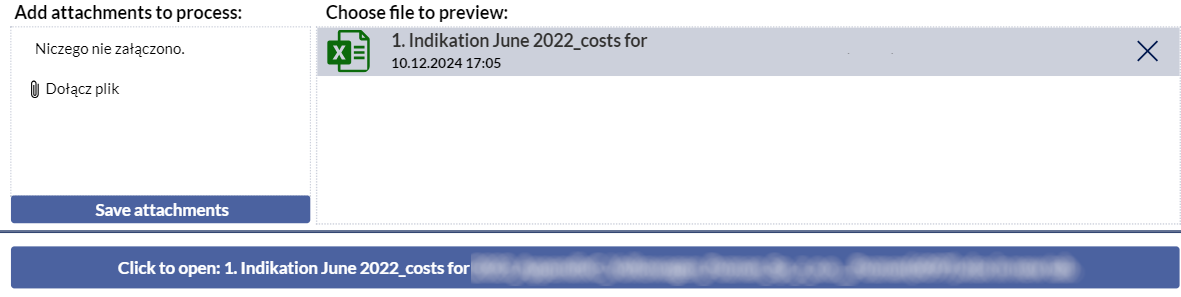
\includegraphics[width=\textwidth]
    {figures/SaveAttachmentsForm.png}
    \caption{Formularz zapisu pliku}    
    \label{fig:saveattachmentsform}
\end{figure}

Wybór elementu z listy \emph{Choose file to preview} umożliwia wskazanie pliku do dalszego przetwarzania. Selekcja pozycji z listy automatycznie inicjuje wykonanie opisanego wcześniej skryptu, którego celem jest pozyskanie aktualnego zestawu nagłówków. Należy podkreślić, że ten sam proces zachodzi również podczas inicjalizacji aplikacji. 
Funkcjonalność podglądu, zaimplementowana w postaci przycisku umiejscowionego poniżej głównych elementów sterujących, umożliwia otwarcie wybranego pliku w nowej karcie przeglądarki. Jest to szczególnie istotne w kontekście weryfikacji poprawności danych oraz walidacji struktury kolumn. \end{comment}